\documentclass{article}

\usepackage[a4paper,left=1in,right=1in,top=1in,bottom=1in,footskip=.25in]{geometry}
\usepackage{listings}
\usepackage{lipsum}
\usepackage{graphicx}
\usepackage{afterpage}
\usepackage{xcolor}
\usepackage{fancyhdr}
\usepackage{float}
\usepackage{helvet}
\usepackage{url}
\usepackage[toc,page]{appendix}
\usepackage[final]{pdfpages}
\usepackage[hidelinks]{hyperref}

\renewcommand{\familydefault}{\sfdefault}

\pagestyle{fancy}

\graphicspath{{../IMAGES/}}

\lstset{
	escapeinside={/*@}{@*/},
	language=Java,	
	basicstyle=\ttfamily\fontsize{8.5}{12},
	numbers=left,
	numbersep=2pt,    
	xleftmargin=2pt,
	frame=tb,
	columns=fullflexible,
	showstringspaces=false,
	tabsize=4,
	keepspaces=true,
	showtabs=false,
	showspaces=false,
	morekeywords={inline,public,class,private,protected,struct},
	captionpos=b,
	lineskip=-0.4em,
	aboveskip=10pt,
	extendedchars=true,
	breaklines=true,
	prebreak = \raisebox{0ex}[0ex][0ex]{\ensuremath{\hookleftarrow}},
	keywordstyle=\color[rgb]{0,0,1},
	commentstyle=\color[rgb]{0.133,0.545,0.133},
	stringstyle=\color[rgb]{0.627,0.126,0.941},
}

\title{USB/Bluetooth Media Controller\\Final Report}
\author{40056761\\SET09118\\Edinburgh Napier University}
\date{22-04-2016}
\makeatletter
\lhead{SET09118: Final Report}
\rhead{40056761}


\begin{document}
		
	\maketitle
	
	\section*{Abstract}	
		This document is the final report and a summary to the "USB/Bluetooth Media Controller" project started in February [Appendix~\ref{IPP}] [Appendix~\ref{Interim}]. The goal of the project was to research, develop and evaluate a micro-controller based system and mobile application. The purpose of this report is to catalogue the project’s various stages, suggest future work and assert the overall success of the assignment.
	
		%This document is an interim report summarising the current state of the “USB / Bluetooth Media Controller”. The project consists of the research, development and testing of a microcontroller based media controller and a companion mobile application. The purpose of this report is to catalogue the project’s various stages of development and to describe future action.
				
	\pagenumbering{gobble}
				
	\newpage
		
	\pagenumbering{arabic}
		
	\tableofcontents
	
	\listoffigures
	
	\listoftables
	
	\lstlistoflistings
		
	\newpage
		
	\section{Introduction}
		\subsection{Background and Rational}
			The goal for this project was to produce a system that would allow users to interact with their PC media in a more intuitive manner. From tape cassettes to compact discs and finally to digital MP3 files, the way in which media is stored and experienced had changed dramatically over the last twenty years but the way that users interact with their media has remained stagnant.
			
			While playing or pausing media, changing track or altering volume are typically not difficult tasks for most users, it can often be complicated when the media is not in focus or other applications are in use. Many companies have attempted to solve this issue by incorporating media control keys into keyboards, however these buttons are often in hard to reach locations or only work with specific applications.
			
			For the reasons mentioned above, it is clear that a independent media-controller, that supports a multitude of media application would be a popular device for many users that utilize a PC as the main source of their media. One of the key deliverables of this project is the aforementioned media controller, the other is a companion mobile application that will allow users to access media functions while away from the PC or controller.
					
		\subsection{Aims and Deliverables}
			As stated previously, the two major deliverables discussed in this report are; a micro-controller based media controller and an Android mobile application to control said device. The aim of both deliverables is to simplify the way a user interacts with media, and this was a major consideration for design and implementation of the systems.
			
			\paragraph{Media Controller}
				The Media controller is a device that can be connected to a PC via USB, and provide users with a simple,  physical interface with which to interact with their media. 
				
				In terms of functionality, the controller will provide users with the ability to play or pause their music, skip to the next or previous track and raise or lower the volume of the music. These functions are accessible through a set of push buttons, providing tactile feedback to the user.
				
				Basing the system around an Arduino micro-controller \cite{Arduino:online} allows for simple expansion of the project. For instance, additional buttons, switches or potentiometers can be easily added to the system and allow a user to customize the controller and augment its functions.
			
			\paragraph{Mobile Application}
				The media controller was designed to abstract media functions into the simplest interface possible, the Android application attempts to do the same.
				
				The benefit of a mobile application is that it allows a user to interact with their media, even if they are not at their desk. 
				
				The goal of the application's appearance was to keep it as minimal as possible. The reason for this was to ensure the application's design was appealing and keep it as easy-to-use as possible.
				
				In terms of functionality, the Android application will offer a user the same PC media functions as the physical controller, but via a remote, digital interface.
							
			\paragraph{Limitations}
				In an ideal world, a media controller would be able interface with any device, and any media application, allowing for complete control without the need for installation and configuration. Unfortunately, it would be impossible to ensure total functionally on every combination of operating system, hardware and media application, so limitations were imposed to keep the implementation reasonable. MoSCoW was used to determine what was within scope of the project.

			\begin{minipage}{\textwidth}\label{MoSCoW}
				\paragraph{MoSCoW}
					\noindent\\
					\textbf{Must:}
						\begin{itemize}
							\item Media controller functionality on a PC running Windows operating system
							\item Media key support for the Google Play Music application
						\end{itemize}			
					\textbf{Should:}
						\begin{itemize}
							\item Not require proprietary code running on PC to execute commands
						\end{itemize}
					\textbf{Could:}
						\begin{itemize}
							\item No configuration required / plug-n-play support
							\item Support for additional host devices
							\item Support for additional media applications
						\end{itemize}
					\textbf{Won't:}
						\begin{itemize}
							\item IOS or Windows Phone support
						\end{itemize}
				\end{minipage}
				
	\section{Design}
		\subsection{Media-controller Design}
			While it was a simple task to specify what functionality the media-controller would have, it proved much harder to determine the way in which it would be delivered.
			
			\paragraph{Key press scripts}Preliminary research indicated that a common method of allowing a micro-controller execute commands on a PC was through "man-in-the-middle" scripts, such AutoHotkey \cite{AutoHotkey:online} or AutoIt \cite{AutoIt:online}. These programs would be run on a computer, intercept signals from a connected micro-controller and execute the requested command as a simulated keystroke.
			
			While key scripts did provide a solution, they did come with major flaws; Firstly, key scripts would only work with media applications that already support keyboard short-cuts and secondly, the MoSCoW method produced for this project (Section~\ref{MoSCoW}, Page~\pageref{MoSCoW}) stated that propriety programs should be avoided if possible.
			
			When it was determined that Key press scripts would offer only a partial solution to the project, further research was taken to find a superior method.
			
			\paragraph{Human Interface Devices}Peripherals like USB keyboards, game pads and joysticks are all classified as USB Human Interface Devices or HID's \cite{HID:online} \cite{HIDSiliconLab:online}. When a HID is plugged into a PC it transmits a list of hexadecimal values called a usage table \cite{HIDUsagePage:online} to the host PC. Each number in the usage table corresponds to a specific command or function for the host device to carry out. The commands that can be included in the table consist of everthing from printing characters (keyboard) to moving a mouse cursor (track ball), in addition, a number of media controls are available through the use if a HID usage table. 
			
			\begin{figure}[]
				\centering
				\label{fullSystem}
				{\includegraphics*[scale = 0.5]{fullSystem}}
				\caption{The completed media-controller consisting of; micro-controller, Bluetooth module and push-button panel.}
			\end{figure}
			
			\begin{figure}[]
				\centering
				\label{leonardo}
				{\includegraphics*[scale = 0.15]{leonardo}}
				\caption{//ToDo - Write a caption}
			\end{figure}
			
			\begin{figure}[]
				\centering
				\label{breadboard}
				{\includegraphics*[scale = 0.15]{breadboard}}
				\caption{//ToDo - Write a caption}
			\end{figure}
		
		\subsection{Mobile Application Design}
			\lipsum[1]


	\section{Implementation}
		\subsection{Media-controller Implementation}
			\lipsum[1]
			
			\begin{table}[h]
				\centering
				\caption{A usage table of the HID commands utilized by the media-controller}
				\label{usageTable}
				\begin{tabular}{|r|r|r|}
					\hline
					\multicolumn{1}{|l|}{Usage ID} & \multicolumn{1}{l|}{Usage Name} & \multicolumn{1}{l|}{Usage Type} \\ \hline
					0xCD                           & Play/Pause                      & OSC                             \\
					0xB0                           & Play                            & OOC                             \\
					0xB1                           & Pause                           & OOC                             \\
					0xB3                           & Fast Forward                    & OOC                             \\
					0xB4                           & Rewind                          & OOC                             \\
					0xB5                           & Scan Next Track                 & OSC                             \\
					0xB6                           & Scan Previous Track             & OSC                             \\
					0xB7                           & Stop                            & OSC                             \\
					0xE2                           & Mute                            & OOC                             \\
					0xE9                           & Volume Increment                & RTC                             \\
					0xEA                           & Volume Decrement                & RTC                             \\ \hline
				\end{tabular}
			\end{table}
			
		\subsection{Mobile Application Implementation}
			\lipsum[1]
			
	\section{Results}
		\subsection{Achievements}
			\lipsum[1]
			
		\subsection{Recommendations}
			\lipsum[1]
			
	\section{Future Work}
		\lipsum[1]
	
	\section{Conclusion}
		\lipsum[1]
		
	\section{Evaluation of Achievement}
		\lipsum[1]
		
	\addcontentsline{toc}{section}{References}
			
	\bibliographystyle{ieeetran}
	
	\bibliography{final}

	\newpage

	\begin{appendices}

		\section{Arduino Media-Controller Source Code}
			\lstinputlisting[caption = mediaController\_debounce.ino, nolol]{../../ARDUINO/mediaController_debounce/mediaController_debounce.ino}
			\newpage
			
		\section{Arduino Media Key Library Source Code}
			\lstinputlisting[title = Media.h, nolol]{../../ARDUINO/Media/Media.h}
			\newpage
			\lstinputlisting[title = Media.cpp, nolol]{../../ARDUINO/Media/Media.cpp}
			\newpage
			
		\section{Android Application Source code}
			\lstinputlisting[title = MainActivity.java, nolol]{../../ANDROID/MediaController/app/src/main/java/uk/co/sam/mediacontroller/MainActivity.java}
			\newpage
			
			\lstinputlisting[title = BluetoothHandler.java, nolol]{../../ANDROID/MediaController/app/src/main/java/uk/co/sam/mediacontroller/BluetoothHandler.java}
			
			
		\section{Bluetooth Connection Activity Diagram}
			\begin{figure}[H]
				\centering
				\label{AppBtActivity}
				\includegraphics*[scale = 0.75]{applicationConnectionActivity}
				\title{\\An activity diagram depicting the mobile application Bluetooth connection process.}
			\end{figure}
			
		\section{Arduino Leonardo Data Sheet}
		\begin{figure}[H]
			\centering
			\label{LeoDatasheet}
			\includegraphics*[scale = 0.75,angle=90]{ArduinoLeonardoDataSheet}
			\title{\\The Data sheet of the Arduino Leonardo Micro-controller.}
		\end{figure}
					
		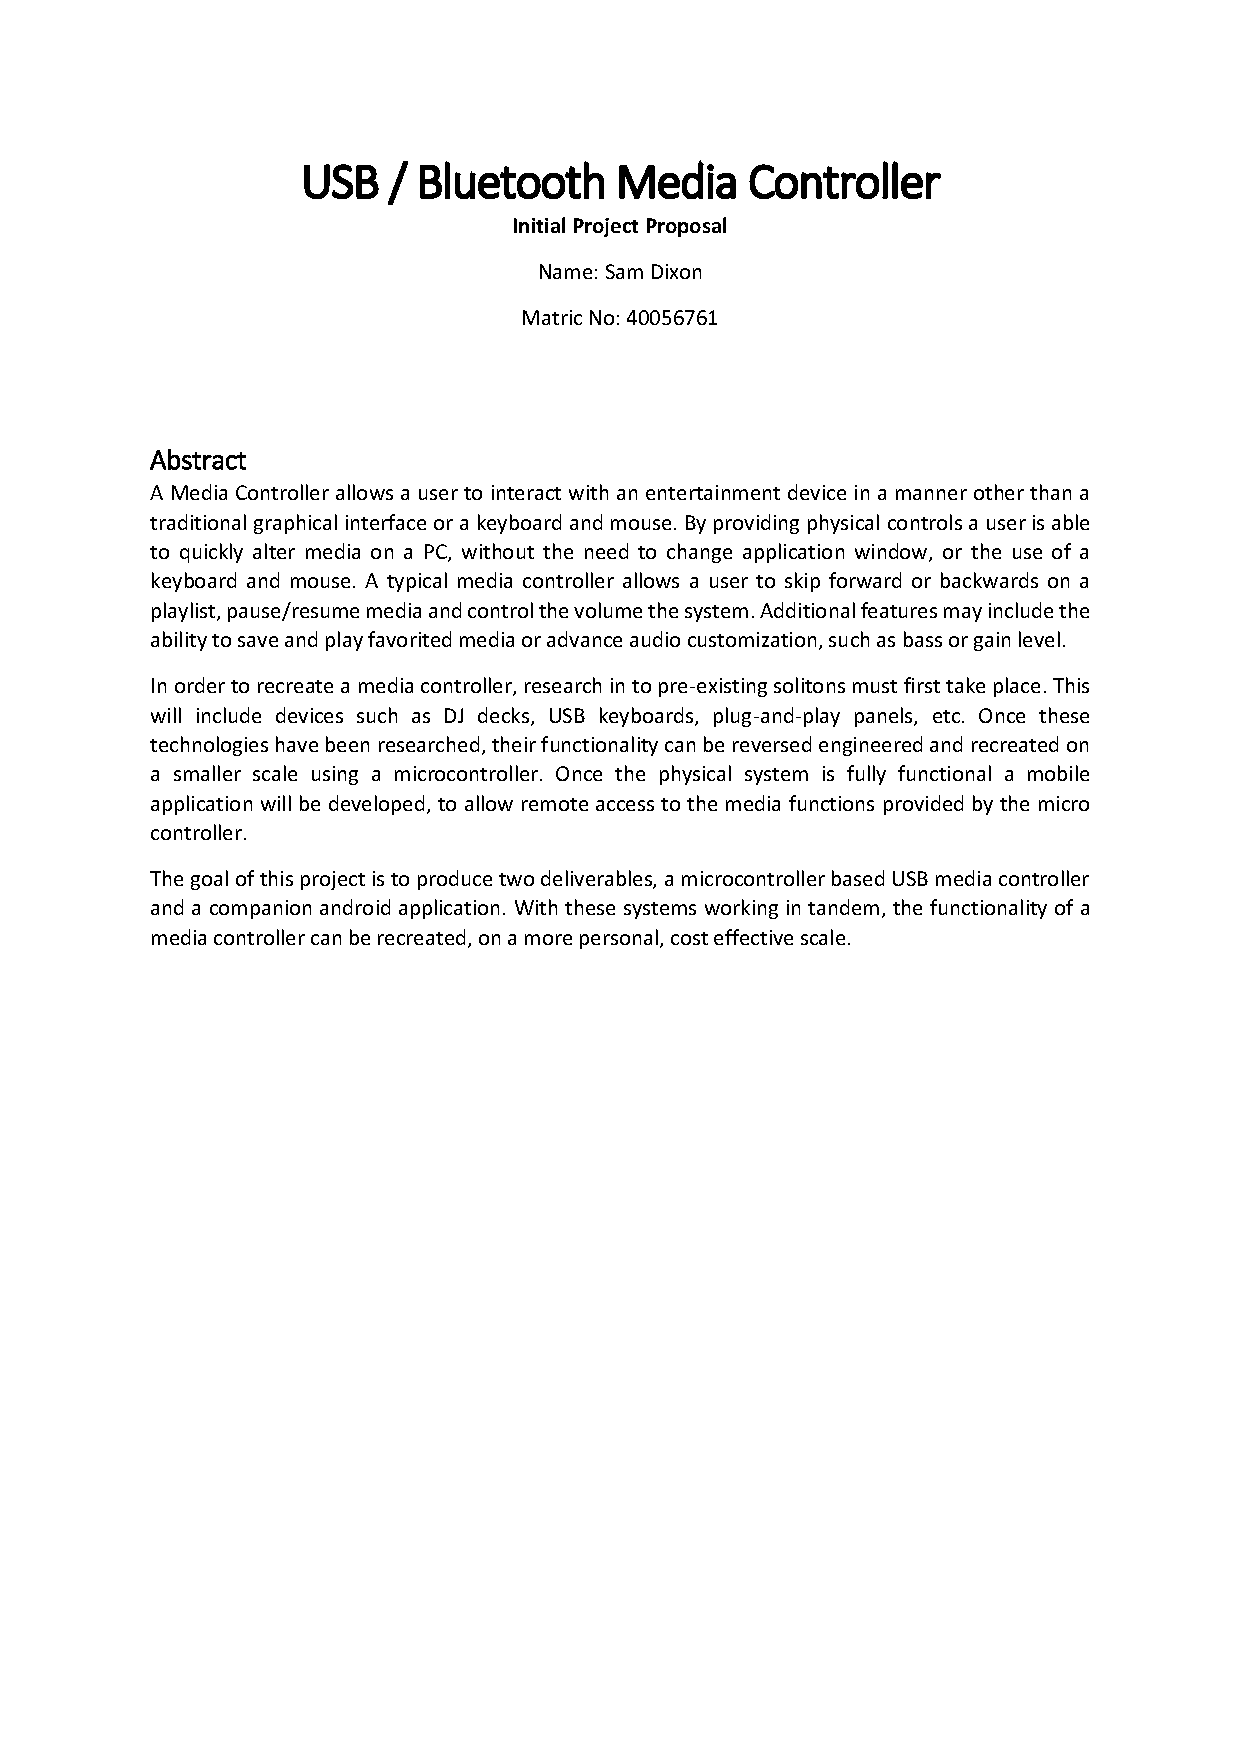
\includepdf[scale = 0.8, pages=1,pagecommand=\section{Initial Project Proposal}\label{IPP}]{../IPP/SET09118_IPP.pdf}
		\includepdf[scale = 0.8, pages=2-,pagecommand={}]{../IPP/SET09118_IPP.pdf}
		\newpage
	
		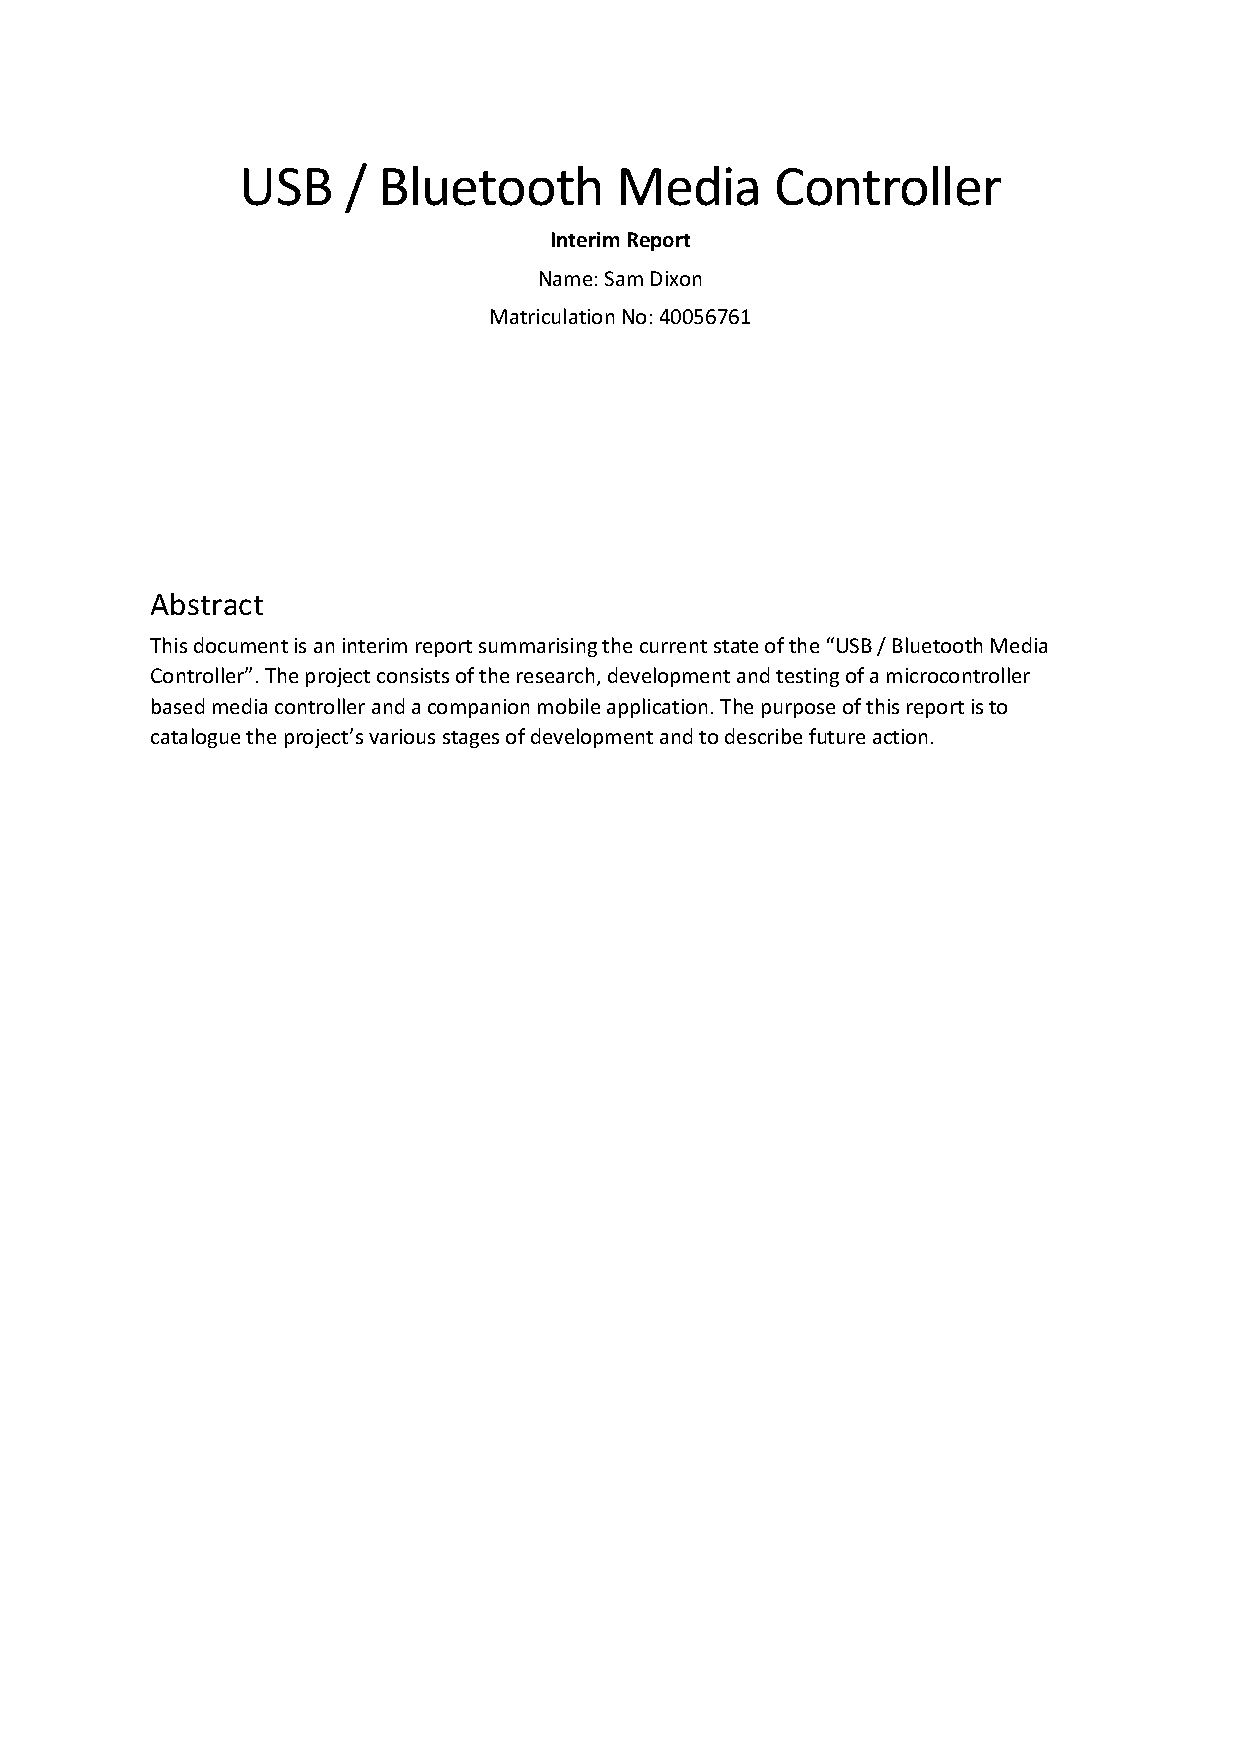
\includepdf[scale = 0.8, pages=1,pagecommand=\section{Interim Report}\label{Interim}]{../INTERIM/SET09118_INTERIM.pdf}
		\includepdf[scale = 0.8, pages=2-,pagecommand={}]{../INTERIM/SET09118_INTERIM.pdf}
		\newpage	

		 		
	\end{appendices}

\end{document}